\section{Requirements}
This section emphasises the requirements for the project, given by the customer
Refslevbæk Bryghus A/S, as it aims to clarify what the customer wants and how
the group is including those requirements in the system. 

\subsection{Overall Requirements Specification}
To make sure all the requirements from the customer are included in the project,
and to give a brief summary of the requirements, a summary of is made.

\subsubsection{Summary of requirements}
The group's proposed solution will adhere to the requirements given by the
brewery Refslevbæk Bryghus A/S, which can be seen in the project description.

The manufacturing execution system, MES, must be able to control the brewery’s 
production. It must be able to start and stop the production line, as well as
monitor the production and collect data from the production line. The data must
be stored for further analysis. The MES must be able to keep track of the
batches that the new machine is producing, as well as collect various data from
the machine that is associated with the current batch number. After a finished
batch production, the MES must be able to produce a batch report. The report
must contain the following.

\begin{itemize}
    \item This Batch ID
    \item Product type
    \item Amount of products (total, defect and acceptable)
    \item Amount of time used in the different states
    \item Logging of temperature over the production time
    \item Logging of humidity over the production time
\end{itemize}

The MES must be able to monitor the production and display live relevant data
from the machine. The system must have a
visualisation that can be accessed and used to display production data. The
system must be able to collect the necessary data from the machine and calculate
the overall equipment effectiveness, OEE, of the machine. The OEE must
be available to be displayed by the system. The system must be able to estimate
the error function associated with the different product types. The system must
be able to find the optimal production speed for each product type, based on an
error simulation and the appertaining graph upon which the error simulation is
built.

\subsubsection{List of requirements}
Below, in Table \ref{table:Requirements}, is a list of the above requirements.
These requirements have been prioritised using the MoSCoW method, where M is for
Must have, S is for Should have, C is for could have, and W is for Won't have. 

\begin{table}[H]
    \captionof{table}{List of requirements} 
    \begin{tabularx}{\textwidth}{|>{\RaggedRight}p{1cm}|>{\RaggedRight}p{4cm}|>{\RaggedRight}X|>{\RaggedRight}p{1cm}|}
        \hline
        \textbf{ID} & \textbf{Name} & \textbf{Description} & \textbf{Prio} \\
        \hline
        R01 & Control production line & Control the brewery's production & M \\
        \hline
        R02 & Control production line & Start/stop production line & M \\
        \hline
        R03 & Monitor production & Monitor data from the production line & M \\
        \hline
        R04 & Monitor production & Store the collected data for further analysis & M \\
        \hline
        R05 & Administer batches & Keep track of produced batches (batch ID) & M \\
        \hline
        R06 & Store batch info & Collect various data associated with current batch number from the machine & M \\
        \hline
        R07 & Batch report & Produce a batch report (PDF/dashboard style format) & M \\
        \hline
        R08 & Live data & Monitor and display live relevant data from the machine & M \\
        \hline
        R9 & Visualisation & Visualisation that can be accessed and used to display the production data & M \\
        \hline
        R10 & OEE & Collect necessary data from the machine and calculate the OEE. OEE must be available to be displayed by the system & M \\
        \hline
        R11 & Estimate error function & Estimate the error function associated with the products & S \\
        \hline
        R12 & Optimal Production speed & Estimate the optimal production speed for each product type & M \\
        \hline
    \end{tabularx}
    \label{table:Requirements}
\end{table}

\subsection{Selected Detailed Requirements}
Besides the overall requirements, some detailed requirements are also stated by
the customer, which describes how the system should perform. The group made
additional requirements that were found to potentially add quality to the system
to be developed.  

\subsubsection{Functional \& Non-Functional Requirements}
In Table \ref{table:sup_requirements} you can see a description of Functional and
Non-Functional requirements. These requirements have been classified by using
the FURPS+ method.

\begin{table}[H]
    \captionof{table}{Supplementary Requirements} 
    \begin{tabularx}{\textwidth}{|>{\RaggedRight}p{5.25cm}|>{\RaggedRight}p{0.6cm}|>{\RaggedRight}X|}
        \hline
        \textbf{FURPS+}  & \textbf{\#} & \textbf{Demands} \\
        \hline
        Functionality  	& S01 & Improve the beer machine by increasing quantity while maintaining quality \\
        \hline
        Usability      	& S02 & Documentation on usage of the REST API \\
        \hline
        Reliability    	& S03 & On server reboot, the application will automatically restart \\
        \hline
        Performance    	& S04 & Max response time (API: 400 ms) \\
        \hline
        Supportability 	& S05 & Minimum browser versions (JavaScript version 6)\\
        \hline
        Design constraints 	& S06 & Na \\
        \hline
        \multirow{5}{*}{Implementation requirements} & S08 & Should be controlled via MES\\
        \cline{2-3}
                & S08 & MES should be able to keep track of Batches\\
        \cline{2-3}
                & S09 & Monitor production (Live data)\\
        \cline{2-3}
                & S10 & Estimate error function\\
        \cline{2-3}
                & S11 & Optimal production speed\\
        \hline
        \multirow{14}{*}{Interface requirements } & S12 & Show OEE \\
        \cline{2-3}
                & S13 & Show Batch Report that include:
            \begin{itemize}
                \item Batch ID
                \item Product type
                \item Amount of products (total, defect and acceptable)
                \item Amount of time used in the different states
                \item Logging of temperature over the production time
                \item Logging of humidity over the production time
            \end{itemize} \\
        \cline{2-3}
            & S14 & Visualisation \\
        \hline
        Physical requirements & S14 & The group should work with the beer 
        production machine provied by SDU \\
        \hline
    \end{tabularx}
    \label{table:sup_requirements}
\end{table} 

\subsection{Use Cases}
Use cases are written descriptions of how a user will perform different tasks
on a system. They outline the behaviour of a system as it responds to a request from
the user. Each use case is represented as a sequence of steps, beginning with
the user's goal and ending it when that goal is fulfilled. \\

The first step in developing use cases is to determine the actors.


% \begin{table}[ht]
%    \begin{tabularx}{\textwidth}{|>{\RaggedRight}p{3cm}|>{\RaggedRight}X|>{\RaggedRight}p{2.5cm}|}
%     \hline
%     \textbf{Use Case ID}   & \textbf{Name}                                 & \textbf{Definition}\\ \hline
%     UC01                   & Start production line                         & User \\ \hline
%     UC02                   & Stop production line                          & User \\ \hline
%     UC03                   & Monitor and store data from production line   & SCADA \\ \hline
%     UC04                   & Monitor and display relevant data live        & SCADA \\ \hline
%     UC05                   & Create batch report                           & MES \\ \hline
%     UC06                   & Calculate OEE                                 & MES \\ \hline
%     UC07                   & Estimate the error function                   & MES \\ \hline
%     UC08                   & Find optimal production speed                 & MES \\ \hline
%     \end{tabularx}
%     \caption{Use Cases}
%     \label{table:use_cases}
%     \end{table}

\subsubsection{Actor List}
In order to determine who will be able to access the system, the actors are
found. An actor is defined as an external system or user that communicates
with the system. Not every actor can necessarily be found at the given time,
meaning other actors may be found later during development.

The identified actors can be seen in Table \ref{table:actor_list}. With these
actors, a visualisation can be made, depicting how the different actors
communicate with the system.

\begin{table}[H]
    \captionof{table}{Actor list}
     \begin{tabularx}{\textwidth}{|>{\RaggedRight}p{2.5cm}|>{\RaggedRight}p{8cm}|>{\RaggedRight}X|}
     \hline
     \textbf{Actor} 				& \textbf{Description}                                                                                                              				& \textbf{Goal} \\ \hline
     \multirow{2}{*}{User (p)}      & The user represents the worker of the machine. The user will use the control panel to control the machine.                                  		& 	\begin{itemize}
     																																														\item Control machine
     																																														\item Start new batches
     																																													\end{itemize} \\ \hline
     \multirow{2}{*}{BPM (s)}     	& The beer production machine is responsible for supplying data to the MES and producing the beer.       											& \begin{itemize} 
     																																														\item Collect and save data
     																																														\item Communicate between hardware and MES 
     																																									 				\end{itemize} \\ \hline
    \end{tabularx}
    \label{table:actor_list}
\end{table}

\subsubsection{Detailed Use Cases}
When the actors have been determined, use cases can be developed. These use
cases add value because they help explain how the system behaves and which
functions to include when developing the system. As seen below, in Table
\ref{table:usecase_start}, which represents the sequence of steps happening
when a user wants to start the beer production machine. This use case clarifies
the functions needed to fulfil the user's goal to start the production machine.
The remaining detailed use cases can be seen in appendix \ref{app:usecases}.

% start production
\begin{table}[H]
    \captionof{table}{Production Control: Start machine}
    \begin{tabularx}{\textwidth}{|>{\RaggedRight}X|}
        \hline
        \textbf{ID:} UC01  \\
        \hline
        \textbf{Primary actor:} The user \\
        \hline
        \textbf{Secondary actor:} Beer production machine \\
        \hline
        \textbf{Short description:} The MES must be able to start the brewery's
        production \\
        \hline
        \textbf{Pre conditions:} The beer production machine needs to be in
        ready mode, that is, not producing beer. \\
        \hline
        \textbf{Main flow:} \\
        	1. This use case starts when a user wants to start the beer
        	production machine. \\
        	2. The user chooses what kind of beer to be produced. \\
        	3. The user sets production speed. \\
        	4. The user sets batch id. \\
        	5. The user sets amount of beers to be produced. \\
        	6. The user presses the start button. \\
        	7. The MES starts the machine. \\
        	8. When the production has finished, the MES stores data from the
        	production. \\

		\hline
        \textbf{post conditions:} The beer production machine is turned on \\
        \hline
        \textbf{Alternative flow:} \\
        	Step 8: If the machine does not complete the production (for various
        	reasons) the production stops and stores the data from the machine
        	and the user receives an error message. \\
        \hline
    \end{tabularx}
    \label{table:usecase_start}
\end{table}

\subsubsection{Use Case Diagram}
Below, in Figure \ref{figure:ucdiagram}, an overview of the use cases for the
MES can be seen.

\begin{figure}[ht]
	\centering 
	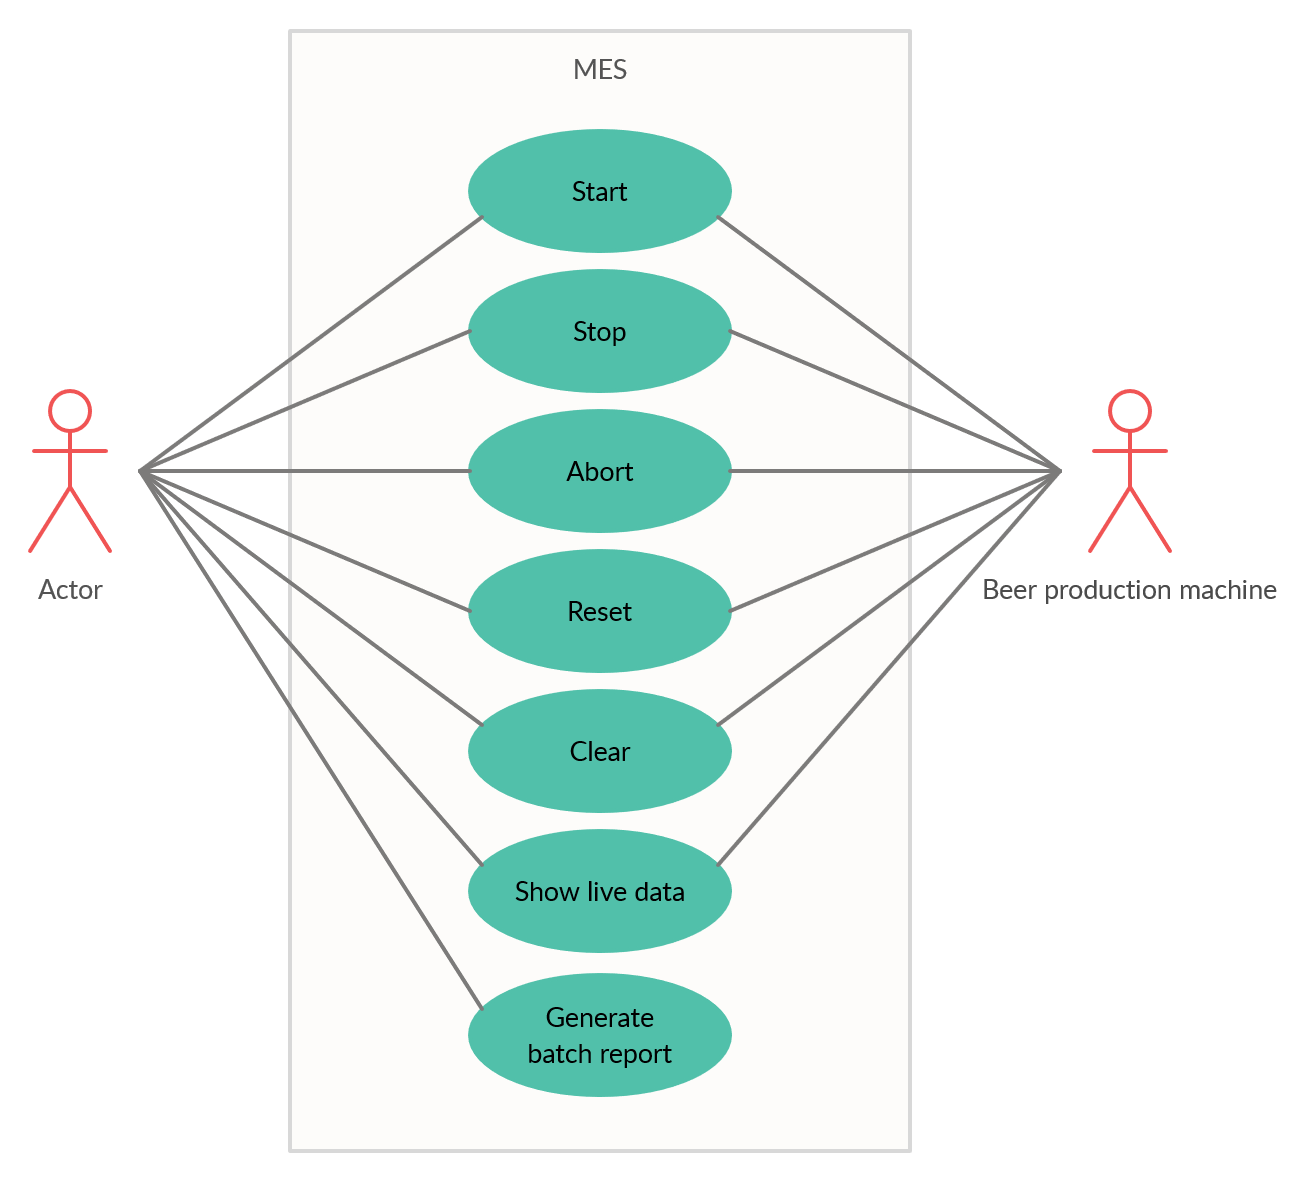
\includegraphics[scale=0.3]{images/ucdiagram.png}
	\caption{Use case diagram}
	\label{figure:ucdiagram} 
\end{figure}
